\begin{figure}[htbp]
\centering
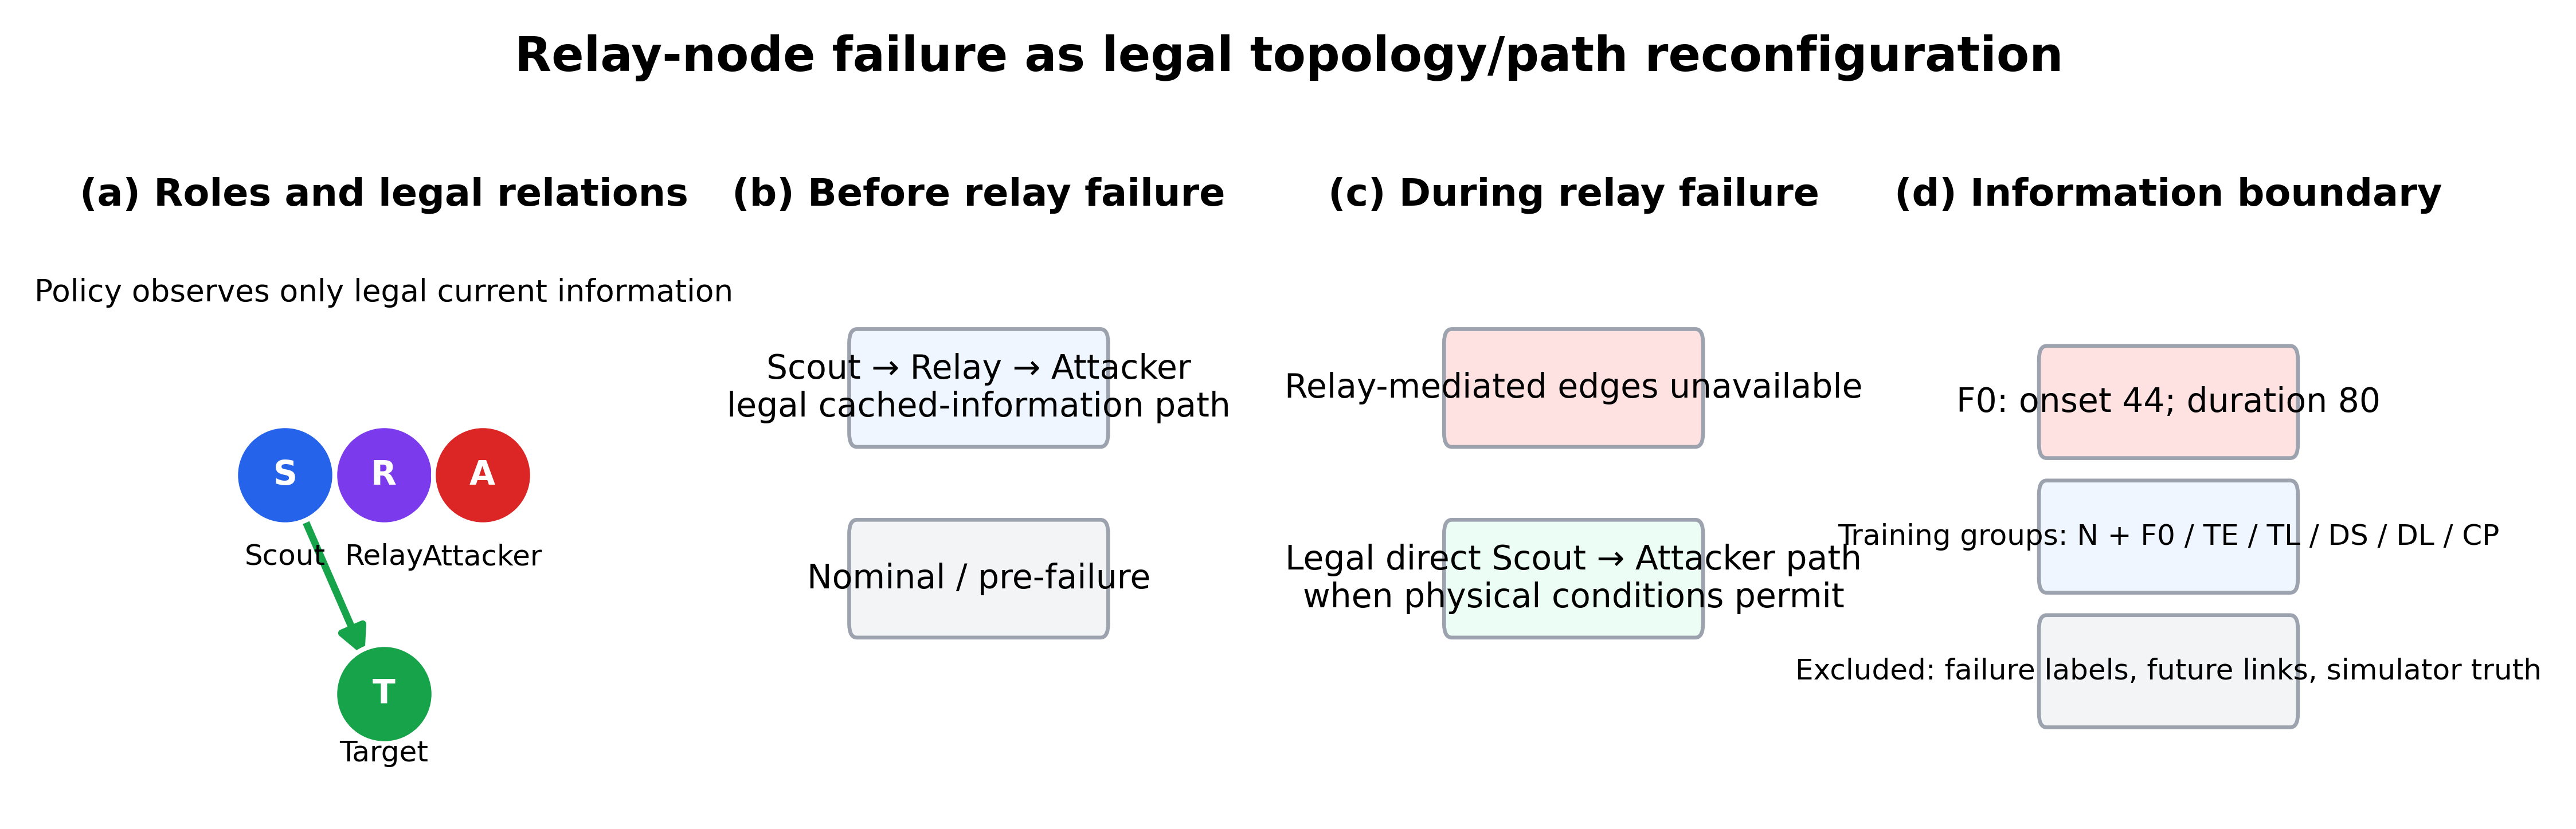
\includegraphics[width=\linewidth]{../figures/fig1_relay_failure_topology_reconfiguration.png}
\caption{Figure 1. Relay-node failure changes the legal information and task-support path from Scout--Relay--Attacker to a direct Scout--Attacker path when that direct relation remains physically legal. This is a task-topology illustration, not a performance result.}
\label{fig:drtp-1}
\end{figure}
\begin{figure}[htbp]
\centering
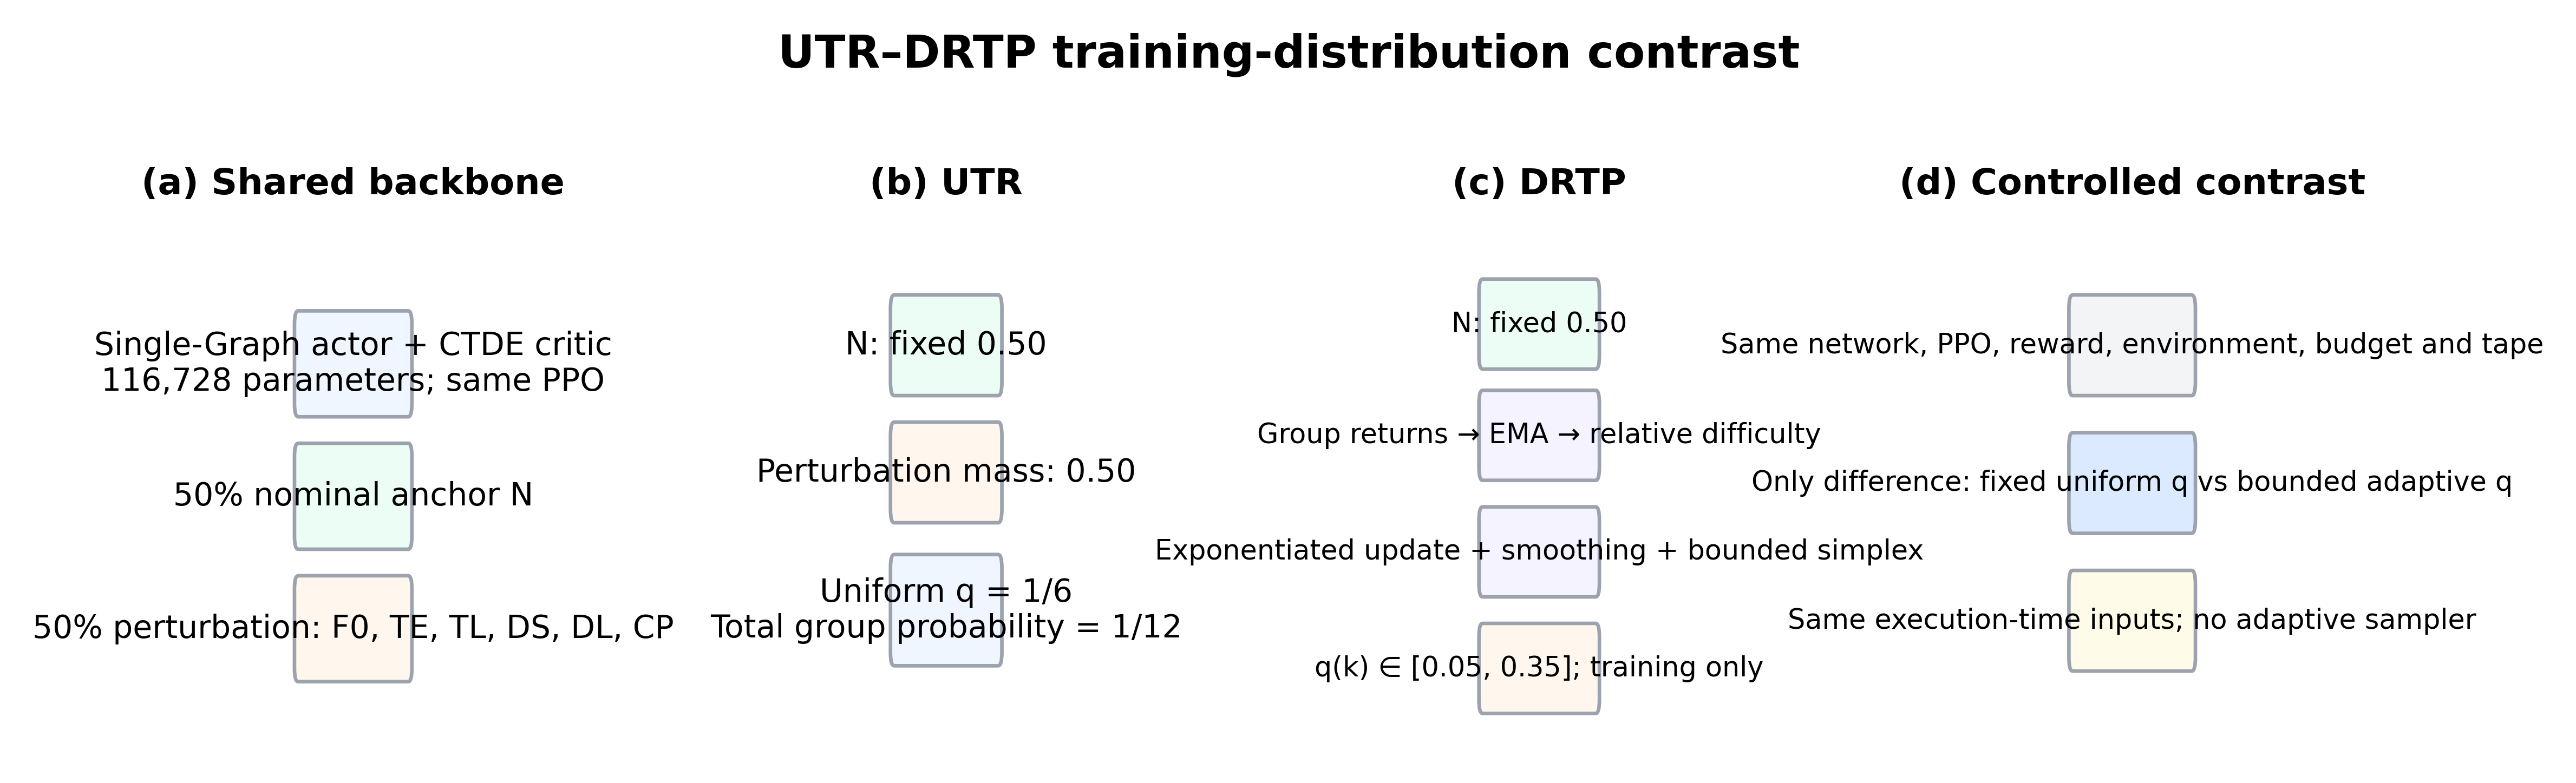
\includegraphics[width=\linewidth]{../figures/fig2_utr_drtp_training_distribution.png}
\caption{Figure 2. UTR and DRTP share the same Single-Graph MAPPO backbone and nominal-condition anchor. DRTP changes only the bounded distribution over the six frozen failure/topology groups during training.}
\label{fig:drtp-2}
\end{figure}
\begin{figure}[htbp]
\centering
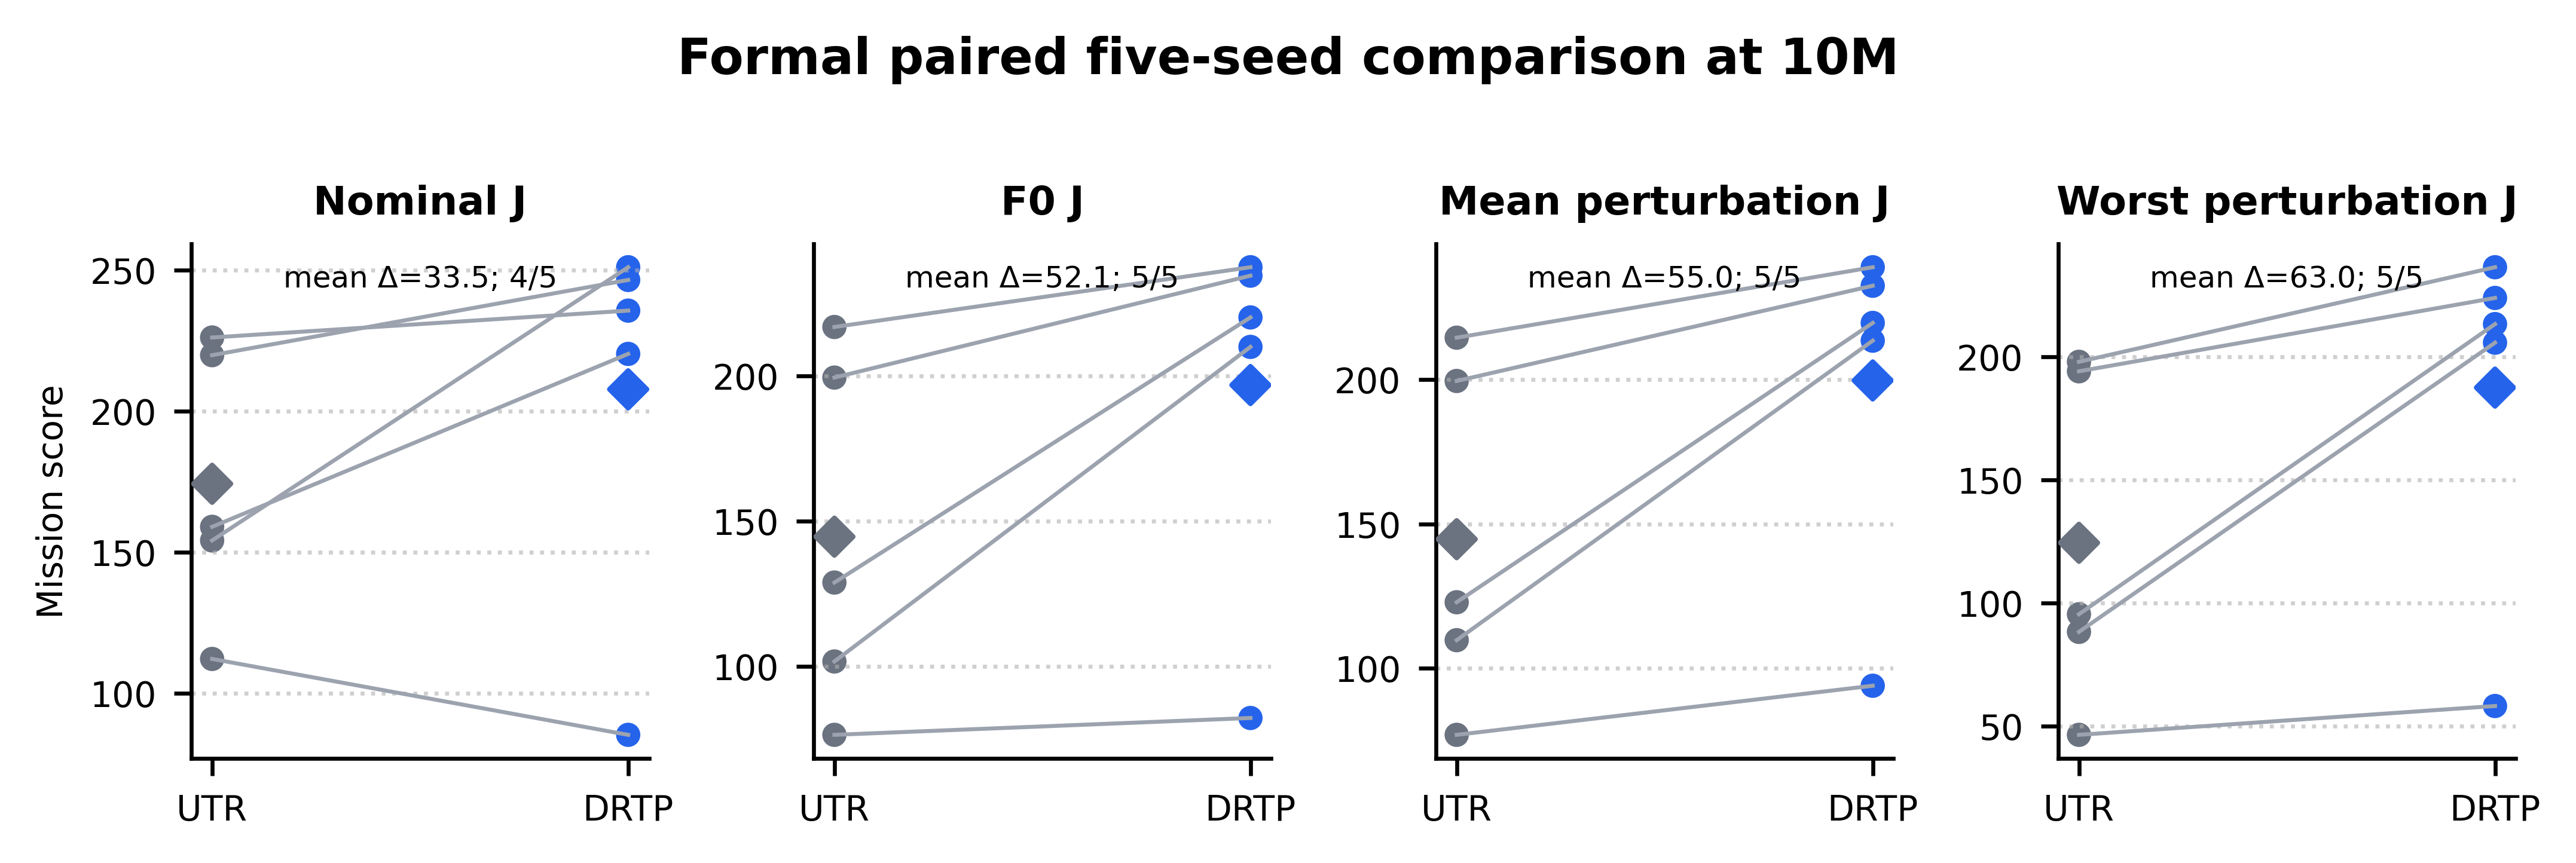
\includegraphics[width=\linewidth]{../figures/fig3_formal_primary_performance.png}
\caption{Figure 3. Formal paired five-seed performance at the common 10M checkpoint. Points show all training seeds; training seed is the independent unit.}
\label{fig:drtp-3}
\end{figure}
\begin{figure}[htbp]
\centering
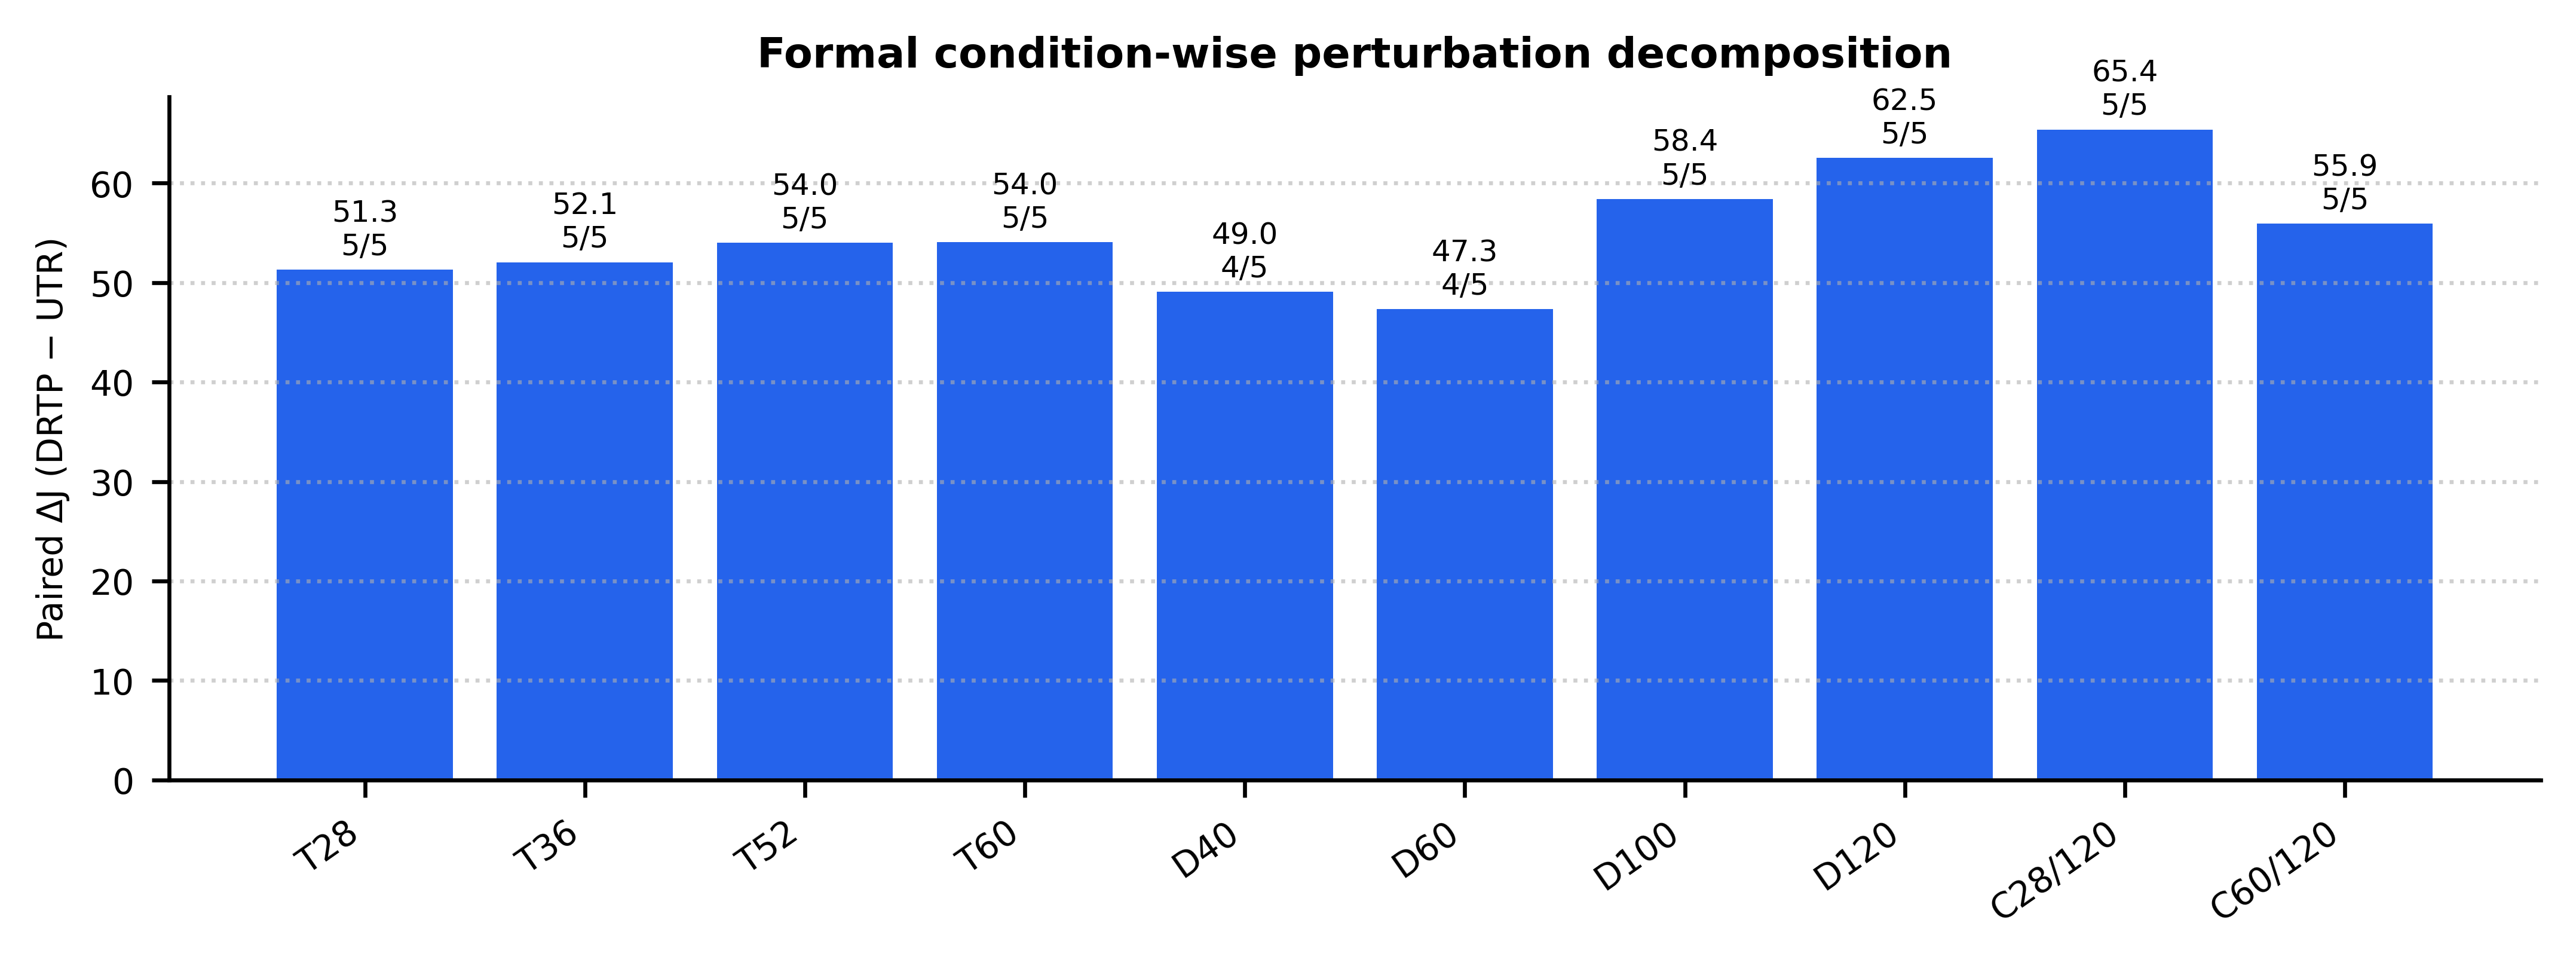
\includegraphics[width=\linewidth]{../figures/fig4_ood_condition_decomposition.png}
\caption{Figure 4. Formal condition-wise decomposition over the ten frozen perturbation members. These members were within training support and are not presented as strict OOD results.}
\label{fig:drtp-4}
\end{figure}
\begin{figure}[htbp]
\centering
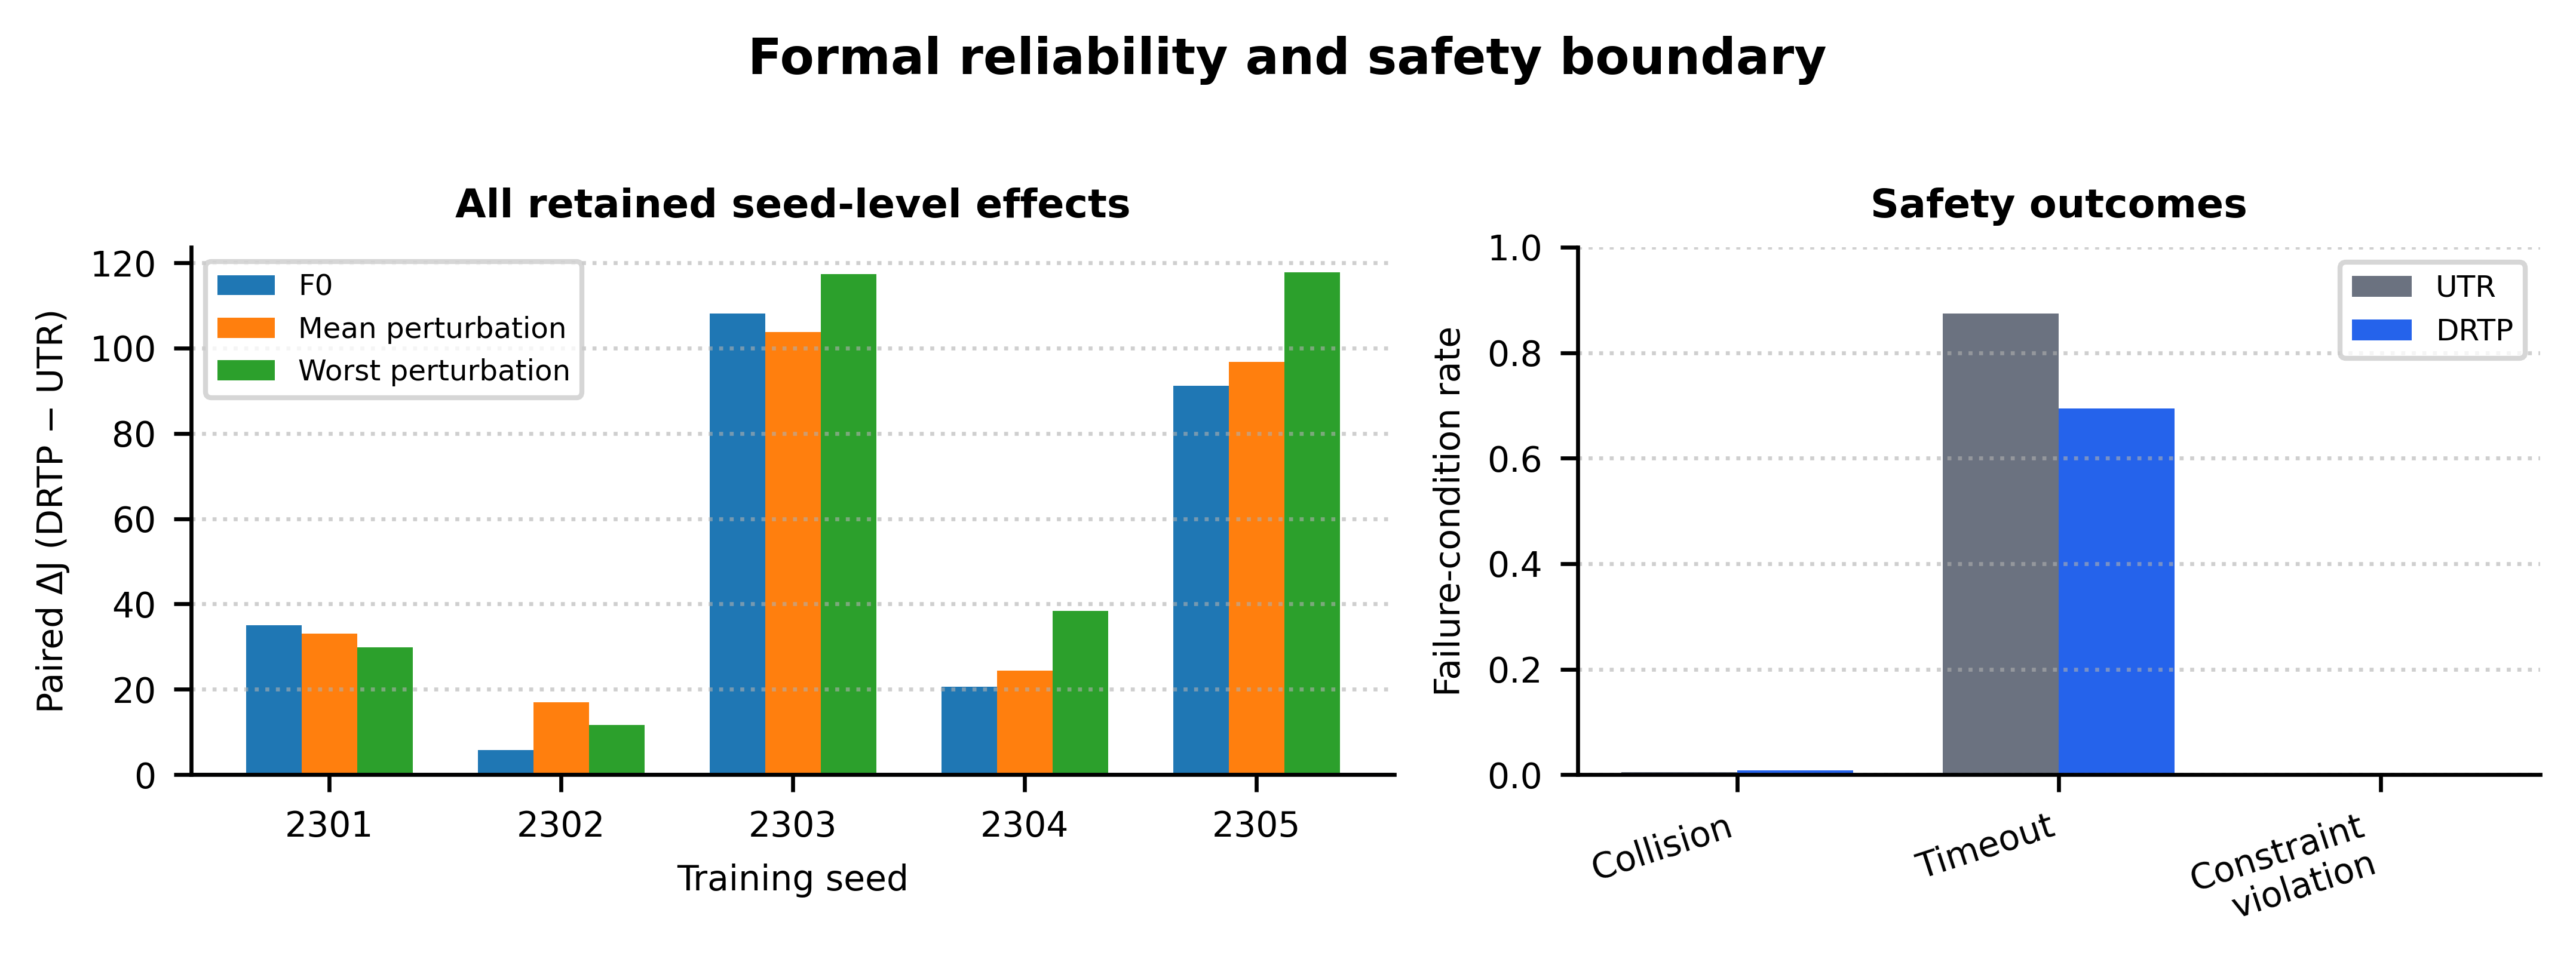
\includegraphics[width=\linewidth]{../figures/fig5_seed_reliability_and_safety.png}
\caption{Figure 5. Formal seed-level reliability and safety audit. The panel separates mission-score outcomes from collision, timeout, and failure-trigger validity.}
\label{fig:drtp-5}
\end{figure}
\begin{figure}[htbp]
\centering
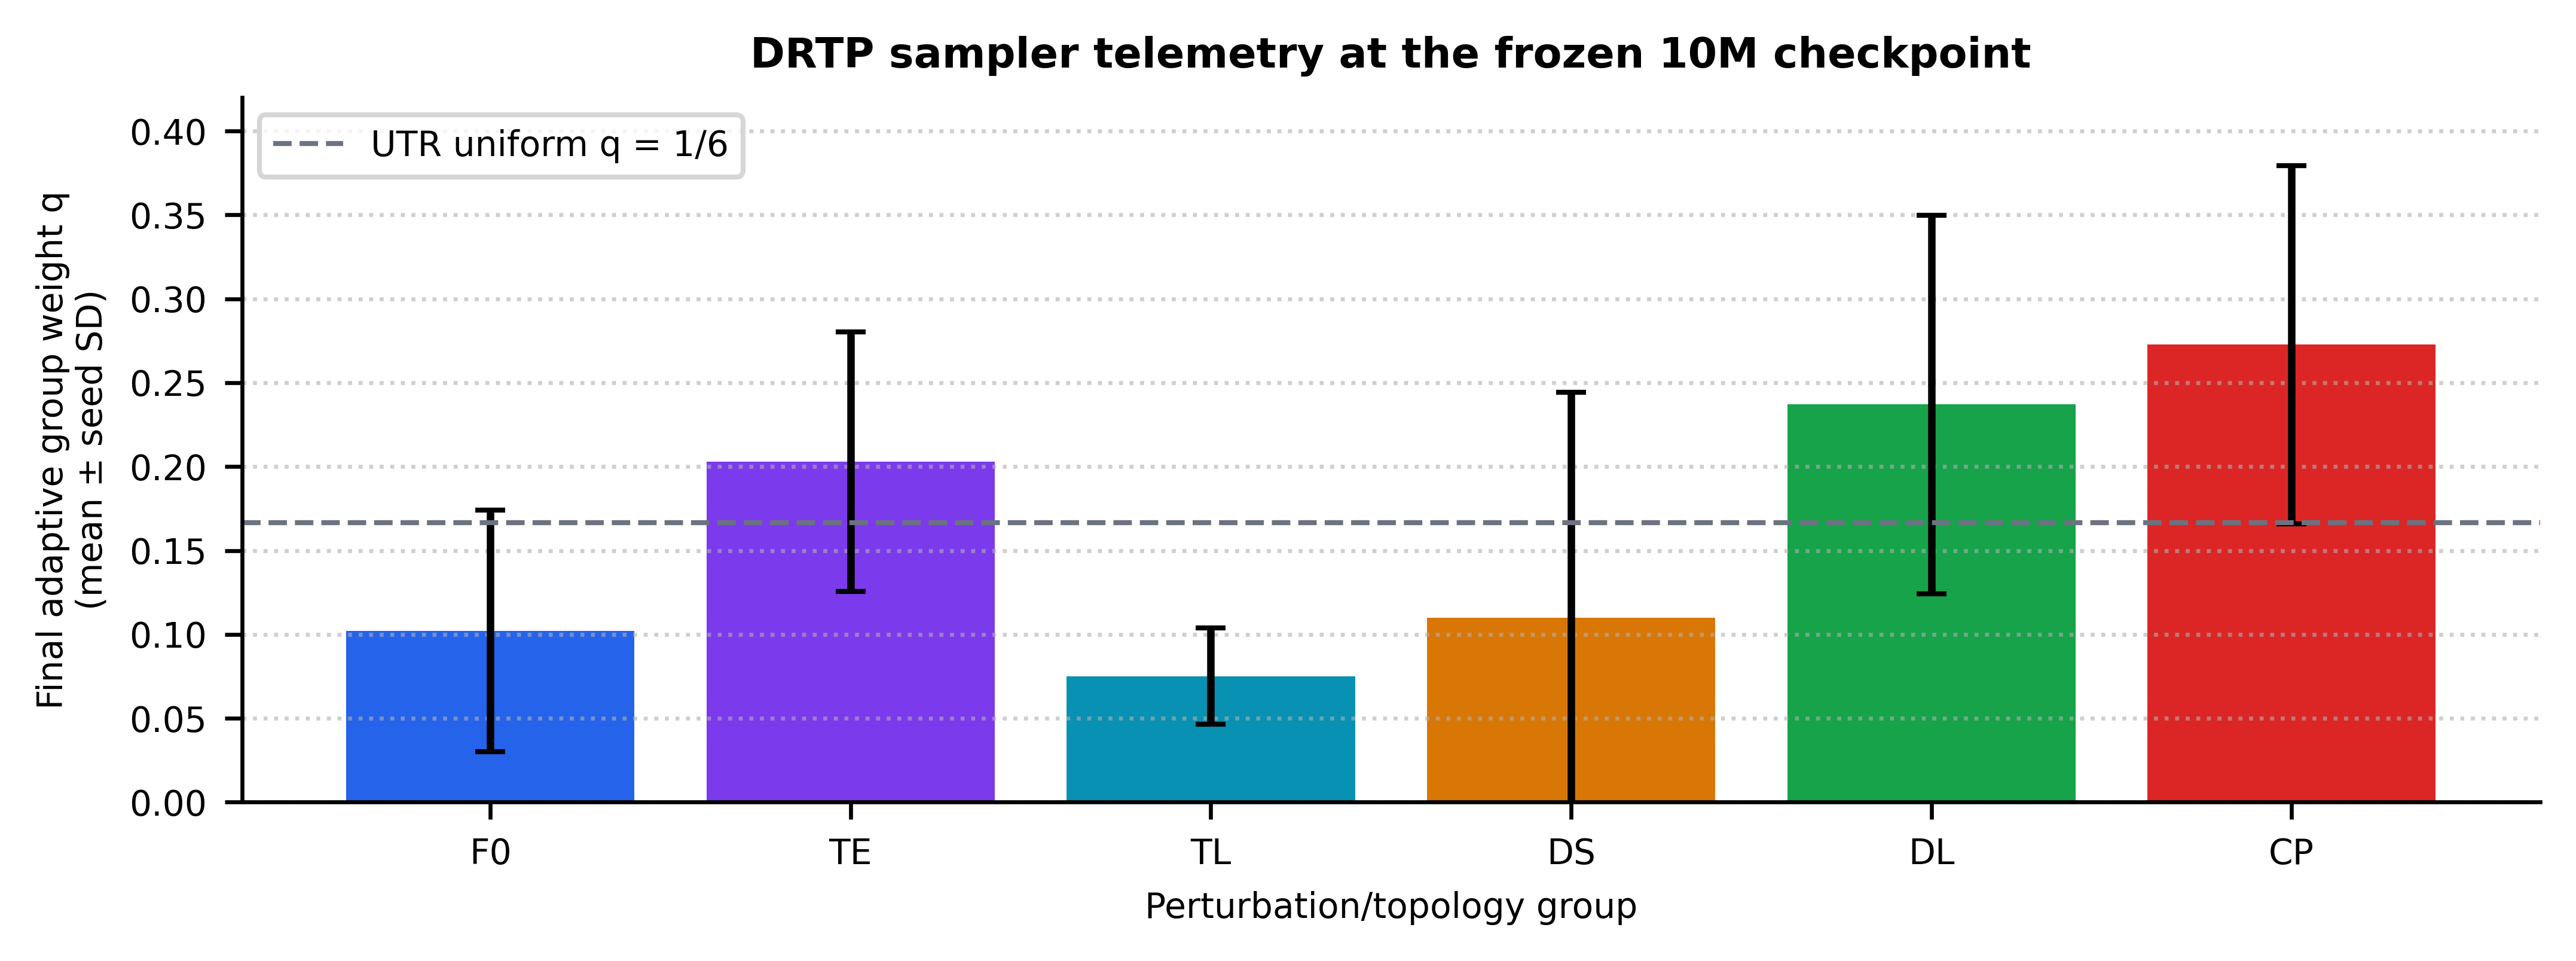
\includegraphics[width=\linewidth]{../figures/fig6_adaptive_weight_telemetry.png}
\caption{Figure 6. DRTP sampler telemetry. These records verify altered training exposure but do not establish a causal policy mechanism.}
\label{fig:drtp-6}
\end{figure}
\begin{figure}[htbp]
\centering
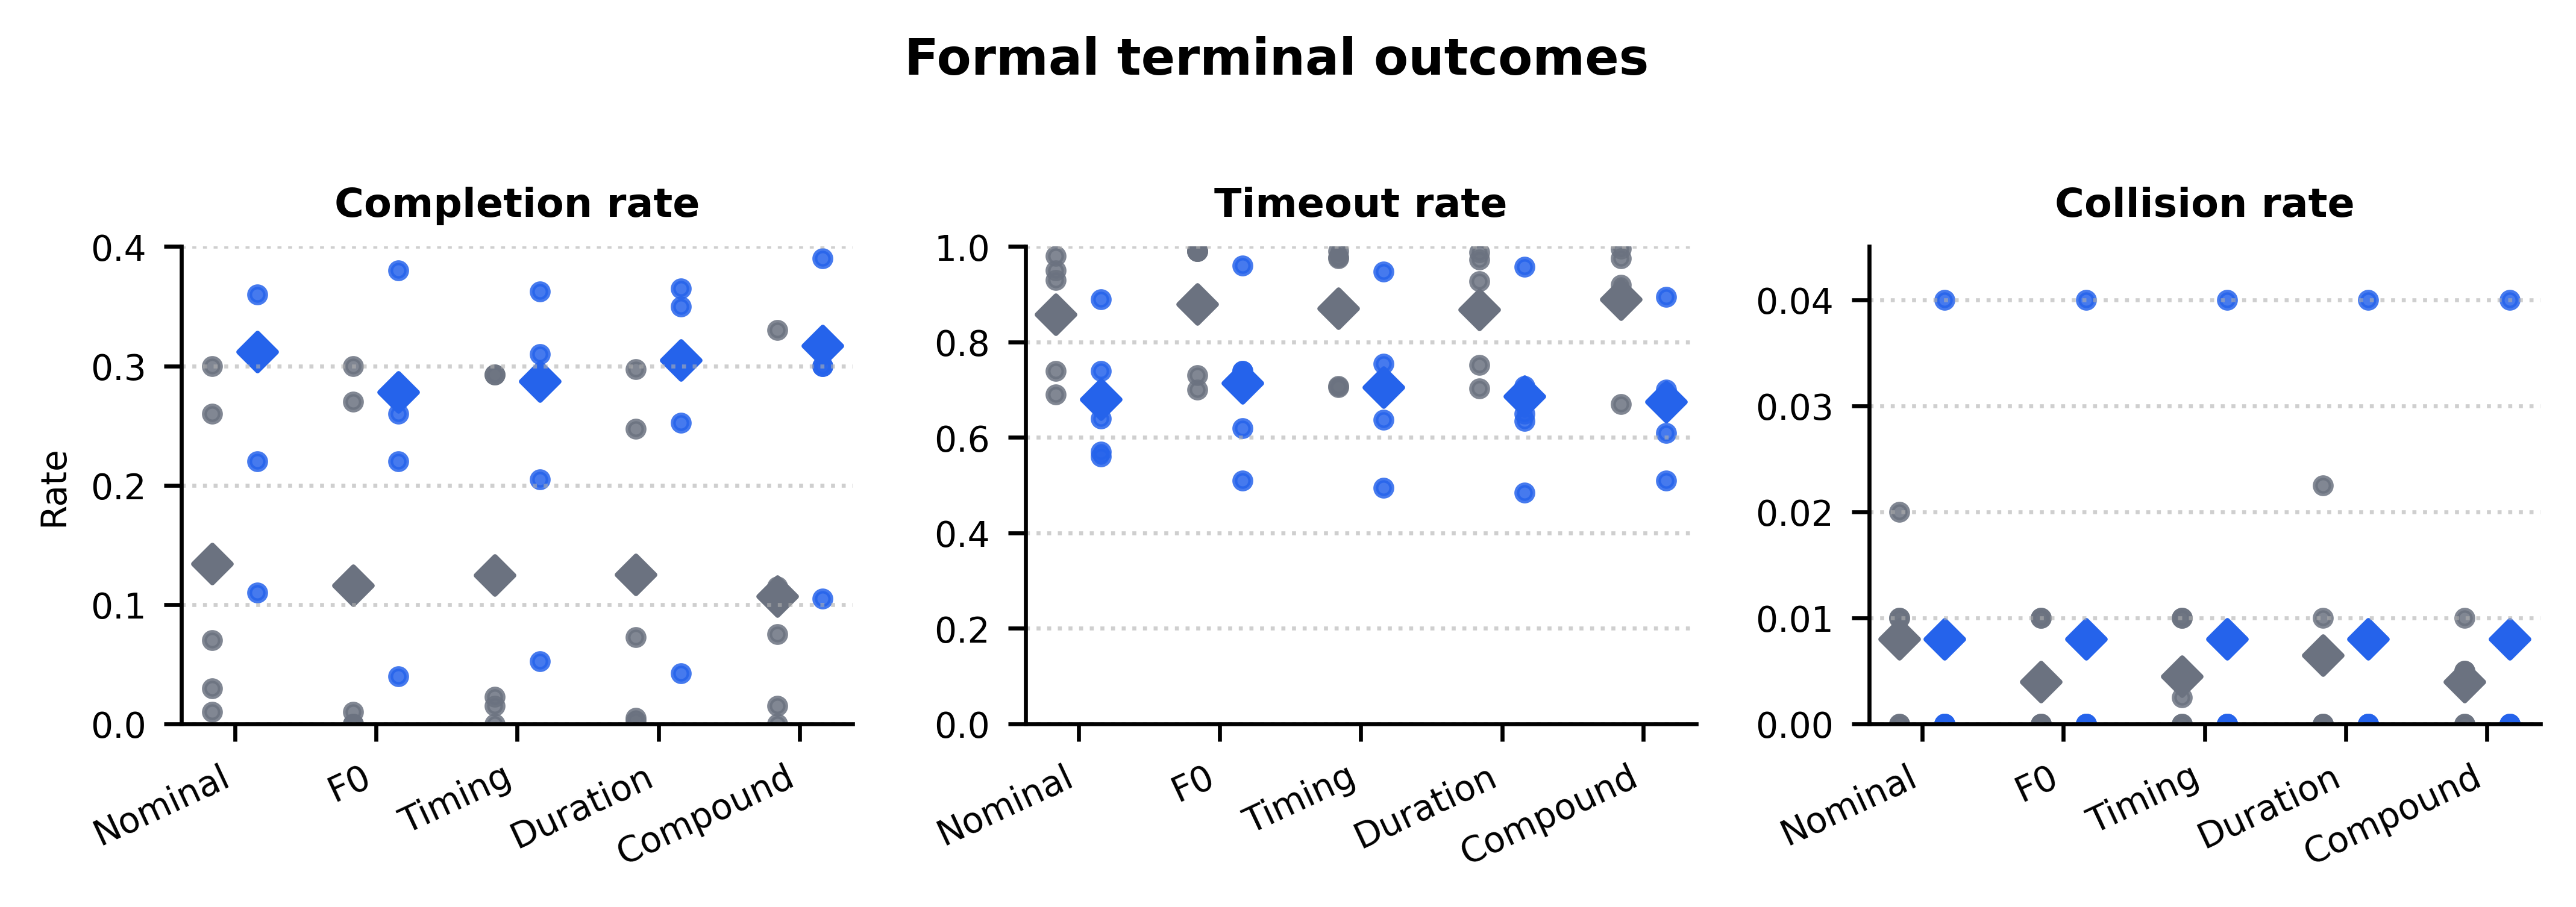
\includegraphics[width=\linewidth]{../figures/fig7_formal_terminal_outcomes.png}
\caption{Figure 7. Formal terminal outcomes. Mission-score gains coincide with greater completion and lower timeout, while collision is reported separately as a trade-off.}
\label{fig:drtp-7}
\end{figure}
